\section{Diogenes in a nutshell}

In this section we show the main features of our tools.
%
\hidden{Firstly, we give an overview of the possible \coco processes
that you can write within Eclipse. 
Then, we present Diogenes, our verification tool for java programs.}



\paragraph{Contracts.}
A contract describes the intended behaviour of a
participant involved in a session.  We use first-order binary session
types~\cite{Honda98esop} as contracts. 
% Session types are terms
%of a process algebra featuring internal/external choice, and
%recursion.

Suppose we want to model a store which waits for an \atom{order},
then sends either the corresponding \atom{amount} or an \atom{abort} message.
The answer may depend on an external service, \eg an insurance company,
which waits for a \atom{req}est, then it answers \atom{ok} or \atom{no}.
%
In Diogenes, we write these two contracts as follows:
%
\begin{lstlisting}[language=coco,basicstyle=\scriptsize\ttfamily]
contract C { order? string . ( amount! int (+) abort! ) }
contract D { req! string . ( ok? + no? ) }
\end{lstlisting}
Receive actions are followed by the question mark (\code{?}) and grouped
with the symbol \code{+}; similarly, we use the
exclamation mark (\code{!}) and the symbol \code{(+)} for
send actions. If omitted, the type of an action is \code{unit}.

\hidden{The corresponding java contract is
\begin{mdframed}
\begin{minted}[
    fontsize=\scriptsize
    %,linenos
    ]{java}
ContractDefinition C = def("C").setContract(
    externalSum().add("order", Sort.string(), internalSum()
                                              .add("amount", Sort.integer())
                                              .add("abort")));     
ContractDefinition D = def("D").setContract(
    internalSum().add("req", Sort.string(), externalSum().add("ok").add("no")));
\end{minted}
\end{mdframed}
where \code{def()}, \code{externalSum()}, \code{internalSum()} 
are static methods of a factory.
}

\paragraph{Specification.}
A naïve \coco specification of our store is the following
\begin{lstlisting}[
    language=coco,
    basicstyle=\scriptsize\ttfamily,
    numbers=left,
    numbersep=12pt]
specification StoreDishonest {
    tellAndWait x C .
    receive x [
        order? v:string . (
            tellAndWait y D . (
                send y req! v .
                receive y [
                    ok? . send x amount! 100
                    + no? . send x abort!
                    + t . send x abort!]))]
}
\end{lstlisting}

The primitive \inlineCoco{tellAndWait} at line \lineno{2}
advertises the contract \code{C},
and then waits until the session is established
When this happens, the variable \code{x} is bound to the session name.
Then, the store waits to receive an \atom{order}, 
binding it to the variable \code{v} (lines \lineno{3}-\lineno{4}).
Then, the store advertises the contract \code{D}, waits to establish a session
\code{y} (line \lineno{5}) and send a \atom{req}uest (line \lineno{6}) with
the value \code{v}.
Finally, the store waits to receive a response \atom{ok} or \atom{no},
and responds \atom{amount} or \atom{abort} on \code{x}. 
The action \inlineCoco{t} models a timeout 
that covers the case of no response (lines \lineno{7}-\lineno{10}).

Our tool correctly detecteds that the above specification is \emph{dishonest}.
Indeed, if the session \code{y}
is never established, 
the store is stuck at line \lineno{5} 
and cannot fulfil the contract \code{C} at session \code{x}.
Furthermore, what happens if the a response arrive after the timeout?
The store does not consume the input and 
therefore does not respect the contract \code{D}.

A possible way to fix the above specification is the following:
\begin{lstlisting}[
    language=coco,
    basicstyle=\scriptsize\ttfamily,
    numbers=left,
    numbersep=12pt]
specification StoreHonest {
    tellAndWait x C .
    receive x [
        order? v:string . (
            tellRetract y D . (
                send y req! v .
                receive y [
                    ok? . send x amount! 100
                    + no? . send x abort!
                    + t . (send x abort! | receive y [ok? + no?])]) 
            : send x abort!)]
}
\end{lstlisting}
At line \lineno{5} we use the primitive \inlineCoco{tellRetract}
which ensures that if the session \code{x} is not established
within a given deadline (immaterial in the specification)
the contract \code{D} is retracted,
and the control passes to line \lineno{11}.
Finally we change the specification of the timeout branch,
adding a parallel execution of a \inlineCoco{receive}
to consume possible inputs.

\hidden{The specification does not aim to be completed. On refining the implementation,
the user must provide suitable timeout values, and 
the order's amount should be derived in some way.}

\hidden{
The \cref{fig:outline} shows the outline derived from the above specification.

\begin{figure}[H]
\centering
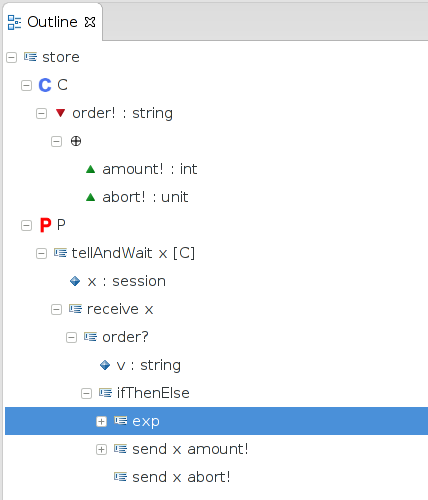
\includegraphics[scale=0.4]{img/outline.png}
\label{fig:outline}
\caption{caption}
\end{figure}
}

\paragraph{Code generation.}
The plugin automatically generates corresponding Maude and Java files.
The former can be used directly within Eclipse to verify its honesty,
exploiting the model-checking tool of~\cite{verifiable};
the latter represents a working java skeleton. 
Considering the honest specification describe above,
Diogenes generates a skeleton that looks like as follows
\begin{mdframed}
\begin{minted}[
    fontsize=\scriptsize
    ,linenos
    ]{java}
public class StoreHonest extends Participant { 
   public void run() {
      Session<TST> x = tellAndWait(C);           // tellAndWait x C
       
      Message msg = x.waitForReceive("order");   // receive c [ order? v:string ]
      String v = msg.getStringValue();
      
      try {
         Session<TST> y = tellAndWait(D, 10000); // tellRetract y D
         y.sendIfAllowed("req", v);
         
         try {                                   // receive y [ok? + no? + t]
            Message msg_1 = y.waitForReceive(10000, "ok", "no");
            switch (msg_1.getLabel()) {                    
               case "ok": x.sendIfAllowed("amount", 100); break;
               case "no": x.sendIfAllowed("abort"); break;                    
            }
         }
         catch (TimeExpiredException e) {        // send x abort! | receive y [ok? + no?] 
            parallel(()->{ x.sendIfAllowed("abort"); });
            parallel(()->{ y.waitForReceive("ok", "no"); });
         }            
      }
      catch(ContractExpiredException e) {
         x.sendIfAllowed("abort");               // : send x abort (line 11)
      }
   }
}
\end{minted}
\end{mdframed}

\hidden{The \inlineCoco{tellRetract} corresponds to perform a tell with
a delay (line \lineno{10}). The successive \code{waitForSession()} blocks until the delay is
expired, throwing a \code{ContractExpiredException} if the session 
was not fused in time (the contract has been retracted).
The timeout \inlineCoco{t} corresponds to a \code{waitForReceived} with a timeout.
The method blocks until a message with label \code{"ok"} or \code{"no"} is received,
or throws a \code{TimeExpiredException} if the timeout expires.}

%\paragraph{Refining the skeleton.}
The order amount is still hardcoded, so we decide to separate its computation
in a separated method, \eg
\begin{mdframed}
\begin{minted}[
    fontsize=\scriptsize
%    ,linenos
    ]{java}
public int getOrderAmount(String order) throws MyException {...}
\end{minted}
\end{mdframed}
and change the number 100 at line \lineno{19} with \code{getOrderAmount(v)}.
The method could read the order's amount from a file or database,
and suppose that each possible exception
is caught and hidden behind \code{MyException}. 

\paragraph{Verification.}
Diogenes allows to verify the honesty of our store
invoking the static method
\code{HonestyChecker.isHonest(StoreHonest.class)}.
%
It returns a value from the enumeration \code{HonestyResult}, that can be
\begin{itemize}
\item \code{HONEST}: the tool was able to extract a \coco model and verify that is honest;
\item \code{DISHONEST}: as above, but the model was dishonest;
\item \code{UNKNOWN}: the tool was unable to extract a model. 
It can be caused by several issues, such as an error of the 
tool or unhandled exceptions within the class under test.
\end{itemize}

Considering \code{StoreHonest} after the refinement provided above,
we need to specify how the method have to be examined by the tool.
The method must be annotated with \code{@SkipMethod (value="<value>")}.
%What happens if the method throws \code{MyException} at runtime.
%The user wants to be sure that its application covers all possible scenarios,
%so we provide the annotation \code{@SkipMethod (value="<value>")}.
Diogenes treats it as follows:
1) retrieves all the declared exceptions;
2) inspects the return type;
3) symbolically considers both the case of a normal termination of the method
(returning the value specified in the annotation, if provided),
and all the possible exceptional terminations.

Once the method is annotated,
Diogenes answers \code{UNKNOWN} and prints the following information
\begin{mdframed}
\begin{minted}[
    fontsize=\scriptsize
%    ,linenos
    ]{java}
error details: MyException: 
    This exception is thrown by the honesty checker. Please catch it!
        at it.unica.co2.store.Store$Phonest.getOrderAmount(Store.java:166)
        at it.unica.co2.store.Store$Phonest.run(Store.java:129)
        at it.unica.co2.honesty.HonestyChecker.runProcess(HonestyChecker.java:182)
\end{minted}
\end{mdframed}
It means that in the case of a method failure,
the program is terminated and the store may be culpable.
Finally, adding \code{x.sendIfAllowed("abort")} when catching the exception,
the program come back \emph{honest}.






